%%%%%%%%%%%%%%%%%%%%%%%%%%%%%%%%%%%%%%%%%%%%%%%%%%%%%%%%%%%%%%%

%
% Welcome to Overleaf --- just edit your LaTeX on the left,
% and we'll compile it for you on the right. If you give 
% someone the link to this page, they can edit at the same
% time. See the help menu above for more info. Enjoy!
%
%%%%%%%%%%%%%%%%%%%%%%%%%%%%%%%%%%%%%%%%%%%%%%%%%%%%%%%%%%%%%%%

%  My thanks to Dana Ernst of Northern Arizona University for sharing 
%    his template with me. This is largely his work.
% --------------------------------------------------------------
% This is all preamble stuff that you don't have to worry about.
% Head down to where it says "Start here"
% --------------------------------------------------------------
 
\documentclass[12pt]{article}
 
\usepackage[margin=1in]{geometry} 
\usepackage{amsmath,amsthm,amssymb}
\usepackage{graphicx}
\usepackage{hyperref}
\usepackage{float}
\usepackage[table,x11names]{xcolor}
\usepackage[lined, linesnumbered]{algorithm2e}
\usepackage{tikz}
\usepackage{xcolor}
\makeatletter
\newenvironment{btHighlight}[1][]
{\begingroup\tikzset{bt@Highlight@par/.style={#1}}\begin{lrbox}{\@tempboxa}}
{\end{lrbox}\bt@HL@box[bt@Highlight@par]{\@tempboxa}\endgroup}

\newcommand\btHL[1][]{%
  \begin{btHighlight}[#1]\bgroup\aftergroup\bt@HL@endenv%
}
\def\bt@HL@endenv{%
  \end{btHighlight}%   
  \egroup
}
\newcommand{\bt@HL@box}[2][]{%
  \tikz[#1]{%
    \pgfpathrectangle{\pgfpoint{1pt}{0pt}}{\pgfpoint{\wd #2}{\ht #2}}%
    \pgfusepath{use as bounding box}%
    \node[anchor=base west, fill=orange!30,outer sep=0pt,inner xsep=1pt, inner ysep=0pt, rounded corners=3pt, minimum height=\ht\strutbox+1pt,#1]{\raisebox{1pt}{\strut}\strut\usebox{#2}};
  }%
}
\makeatother

\usepackage[listings,skins]{tcolorbox}
\tcbset{colback=gray!1!white,colframe=black}




\newenvironment{theorem}[2][Theorem]{\begin{trivlist}
\item[\hskip \labelsep {\bfseries #1}\hskip \labelsep {\bfseries #2.}]}{\end{trivlist}}
\newenvironment{lemma}[2][Lemma]{\begin{trivlist}
\item[\hskip \labelsep {\bfseries #1}\hskip \labelsep {\bfseries #2.}]}{\end{trivlist}}
\newenvironment{conjecture}[2][Conjecture]{\begin{trivlist}
\item[\hskip \labelsep {\bfseries #1}\hskip \labelsep {\bfseries #2.}]}{\end{trivlist}}
\newenvironment{question}[2][Question]{\begin{trivlist}
\item[\hskip \labelsep {\bfseries #1}\hskip \labelsep {\bfseries #2.}]}{\end{trivlist}}
\newenvironment{corollary}[2][Corollary]{\begin{trivlist}
\item[\hskip \labelsep {\bfseries #1}\hskip \labelsep {\bfseries #2.}]}{\end{trivlist}}
\newenvironment{definition}[2][Definition]{\begin{trivlist}
\item[\hskip \labelsep {\bfseries #1}\hskip \labelsep {\bfseries #2.}]}{\end{trivlist}}


\definecolor{commentgreen}{RGB}{176, 176, 176}
\definecolor{rowcolor}{cmyk}{0,0.87,0.68,0.32}
\definecolor{rowcolor2}{cmyk}{ 20, 0, 37, 34}

\definecolor{eminence}{RGB}{108,48,130}
\definecolor{weborange}{RGB}{255,165,0}
\definecolor{frenchplum}{RGB}{129,20,82}
\definecolor{darkgreen}{RGB}{10, 92, 10}


\definecolor{celadon}{rgb}{0.67, 0.88, 0.69}

\definecolor{mGreen}{rgb}{0,0.6,0}
\definecolor{mGray}{rgb}{0.5,0.5,0.5}
\definecolor{mPurple}{rgb}{0.58,0,0.82}
\definecolor{backgroundColour}{rgb}{0.95,0.95,0.92}

\lstdefinestyle{CStyle}{
    commentstyle=\color{mGreen},
    keywordstyle=\color{magenta},
    numberstyle=\tiny\color{mGray},
    stringstyle=\color{mPurple},
    basicstyle=\footnotesize,
    breakatwhitespace=false,         
    breaklines=true,                 
    captionpos=b,                    
    keepspaces=true,                 
    numbers=left,                    
    numbersep=5pt,                  
    showspaces=false,                
    showstringspaces=false,
    showtabs=false,                  
    tabsize=2,
    language=C,
    moredelim=**[is][{\btHL[celadon!40]}]{`}{`}
}

\lstdefinestyle{nccode}{
    numbers=none,
    stepnumber=1,
    numbersep=10pt,
    tabsize=4,
    showspaces=false,
    breaklines=true, 
    showstringspaces=false,
    moredelim=**[is][{\btHL[orange!50]}]{`}{`}
}

\begin{document}
 
% --------------------------------------------------------------
%                         Start here
% --------------------------------------------------------------
 
\title{Assignment 4: GPU Programming} % replace with an appropriate title, choose something shortish & descriptive
\author{Javier Cabrera Arteaga, Deepika Tiwari} % replace with your name, multiple authors go in alphabetical order by last name
 
\maketitle


{%
\centering
FDD3258 - Introduction to High-Performance Computing (GPU module)
\par
}
\hrule
\vspace{.2in}

All source code can be found here \url{XX}.


\section{Exercise 1 - Questions about GPU Architecture}
\begin{enumerate}
    \item \textit{Why did GPUs emerge as suitable hardware for computer graphics (e.g. games)?}\\
    GPUs were traditionally designed to optimize tasks related to image processing and display, and computer graphics. More recently, GPUs are also utilized in deep learning and HPC workloads because of their specialized microcircuits that are can accelerate such tasks and obtain maximum processing speeds. This can be attributed to the large number of ALUs in their processing cores, and hardware-based threads which can handle highly mathematical and highly parallel workloads.
    
    \item \textit{Why do we talk about throughput-oriented architecture when we talk about GPUs?}\\
    GPUs differ from traditional CPUs in their architecture. Traditional CPUs have a latency-oriented architecture, which means that their performance is measured on the basis the time taken to perform an individual task. On the other hand, GPU architecture is throughput-oriented, which means that GPUs aim to maximize the number of tasks performed per unit time. 
    
    \item \textit{List the main differences between GPUs and CPUs in terms of architecture.}\\
    CPU architectures are latency-oriented, whereas GPU architectures are throughput-oriented. In order to achieve low latency, CPU cores have a large Control Unit (CU), and fewer Arithmetic Logical Units (ALUs). This is in contrast to the design of a GPU core, which has many more ALUs and a much smaller CU. Additionally, in CPUs, threads are implemented using software, whereas in the case of GPUs, threads are hardware-based. These architectural differences allow a GPU to complete many more tasks than a CPU in the same amount of time. A single GPU core is simpler in design than a CPU core. It cannot exist in isolation, and usually needs to communicate with a CPU core (called the host) for performing OS tasks. 
    
    \item\textit{Use the Internet to find out and list the number of SMs, the number of cores per SM, the clock frequency, and the size of the memory of the NVIDIA GPU that you plan to use during the course. It might be the GPU of your laptop/workstation, or the GPUs on Tegner (NVIDIA Quadro K420 or NVIDIA Tesla K80). Mention the specific model as well.}\\
    Specifications for the GPUs on Tegner:
    \begin{itemize}
        \item The \textbf{NVIDIA Quadro K420} \footnote{\url{https://www.techpowerup.com/gpu-specs/quadro-k420.c2599}} has 1 SM, with $192$ cores. The clock speed is $876$ MHz and the memory size is $1$ GB.
        \item The \textbf{NVIDIA Tesla K80} \footnote{\url{https://www.nvidia.com/content/dam/en-zz/Solutions/Data-Center/tesla-product-literature/Tesla-K80-BoardSpec-07317-001-v05.pdf}} has 2 SMs, with $2496$ cores each. The base clock speed is $560$ MHz, and the boost clock speed ranges from $562$ MHz to $875$ MHz. The available memory size is  $24$ GB ($12$ GB per core).
    \end{itemize}
    
    \item \textit{Use Google Scholar to find a scientific paper reporting about a work using GPUs in your main domain area (HPC, image processing, machine learning, ...). Report the title, authors, conference name/journal, the GPU type that has been used, and which programming approach has been employed.}
    \begin{itemize}
        \item \textbf{Domain: Software Testing}
        \begin{itemize}
            \item \textit{Title}: Accelarated test execution using GPUs
            \item \textit{Authors}: Ajitha  Rajan, Subodh  Sharma, Peter  Schrammel, Daniel Kroening
            \item \textit{Publication}: ASE '14: Proceedings of the 29th ACM/IEEE international conference on Automated software engineering, September 2014
            \item \textit{DOI}: \url{https://doi.org/10.1145/2642937.2642957}
            \item \textit{GPU specifications}: NVIDIA GTX 670 with 960 cores, a clock speed of 1.07 GHz, and 2 GB memory
            \item \textit{Programming approach}: Parallel execution of software tests  using general-purpose GPUs; One test case with distinct test inputs executed per GPU thread.
        \end{itemize}
      
        \item \textbf{Domain: WebAssembly}
        \begin{itemize}
            \item \textit{Title}:
            \item \textit{Authors}:
            \item \textit{Publication}:
            \item \textit{DOI}:
            \item \textit{GPU specifications}:
            \item \textit{Programming approach}:
        \end{itemize}
    \end{itemize}
\end{enumerate}

\section{Exercise 2 - Bandwidth Test (performed on Tegner)}
\textit{One of the current weaknesses of GPU programming is the link between the host and device (GPU) memories. Measure the bandwidth between host-to-device, device-to-host and device-to-device on Tegner using the bandwidthTest utility. Follow the instructions to run the bandwidth test and answer questions that are at the end of the report. Looking at the results, explain in the report your observations, and why the bandwidth is behaving like that. You can optionally provide a line plot to help your explanation.}\\


The output of \texttt{bandwidthTest} on Tegner is included in \autoref{lst:bandwidthTest}, and \autoref{fig:bandwidthTest} shows the plot for the output of \texttt{bandwidthTest} with the \texttt{--mode=shmoo} flag.

\begin{figure}[H]
\centering
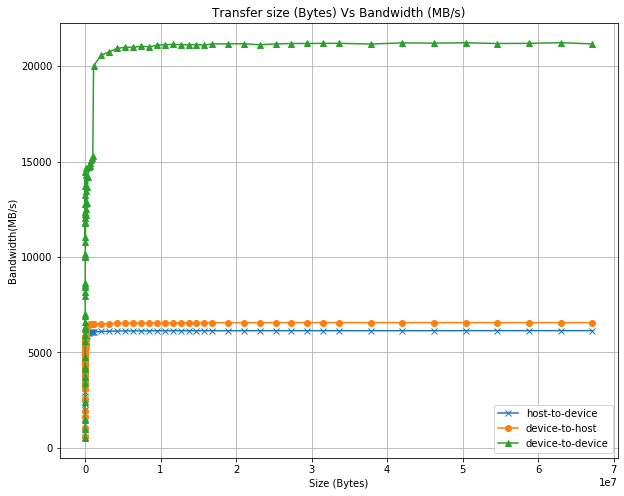
\includegraphics[width=0.8\textwidth]{bandwidthTest.png}
\caption{Transfer Size Vs. Bandwidth with \texttt{bandwidthTest --mode=shmoo} on Tegner}
\label{fig:bandwidthTest}
\end{figure}

\begin{lstlisting}[language=bash, label={lst:bandwidthTest}, caption={bandwidthTest on Tegner}, captionpos=b]

 bash-4.2$ srun -n 1 ./bandwidthTest
[CUDA Bandwidth Test] - Starting...
Running on...

 Device 0: Quadro K420
 Quick Mode

 Host to Device Bandwidth, 1 Device(s)
 PINNED Memory Transfers
   Transfer Size (Bytes)	Bandwidth(MB/s)
   33554432			6152.9

 Device to Host Bandwidth, 1 Device(s)
 PINNED Memory Transfers
   Transfer Size (Bytes)	Bandwidth(MB/s)
   33554432			6553.5

 Device to Device Bandwidth, 1 Device(s)
 PINNED Memory Transfers
   Transfer Size (Bytes)	Bandwidth(MB/s)
   33554432			21287.5

Result = PASS

NOTE: The CUDA Samples are not meant for performance measurements.
Results may vary when GPU Boost is enabled.
\end{lstlisting}

\textbf{From \autoref{fig:bandwidthTest} and \autoref{lst:bandwidthTest}, we can make the following observations}:
\begin{itemize}
    \item Device-to-device transfer is much faster than data transfers between the device and the host. The PCIe bus connects the host CPU to the external GPU. The peak transfer rate between the host and the device is determined by the bandwidth of the bus. There is also additional overhead associated with transfer over the bus.
    \item Device-to-host transfer speeds are slightly higher than host-to-device transfer speeds
    \item The values of bandwidth for all three cases appear to plateau for data sizes around $3223552$ MB ($0.3e7$ in the plot).
\end{itemize}

\section{Exercise 3 - Hello World!}

\begin{lstlisting}[style=CStyle]
#include <stdio.h>
#include <cuda.h>

__global__ void cuda_hello(){
    int myId = blockIdx.x*blockDim.x +  threadIdx.x; // thread indexing
    printf("Hello World! My thread is %d\n", myId);
}

int main() {
  cuda_hello<<<1,256>>>();

  cudaError_t cudaerr = cudaDeviceSynchronize();
  if (cudaerr != cudaSuccess)
    printf("kernel launch failed with error \"%s\".\n",cudaGetErrorString(cudaerr));

  return 0;
}
    \end{lstlisting}
    

\section{Exercise 4 - SAXPY}


\begin{lstlisting}[style=CStyle]
  __global__ void gpu_vector_add(float * __restrict__ x, float * __restrict__  y, int n, float A){
    
   int index = blockIdx.x*blockDim.x + threadIdx.x;
   if (index < n) y[index] = A*x[index] + y[index];
        
} 
\end{lstlisting}

Each thread calculates its own index.

\begin{figure}[H]
\centering
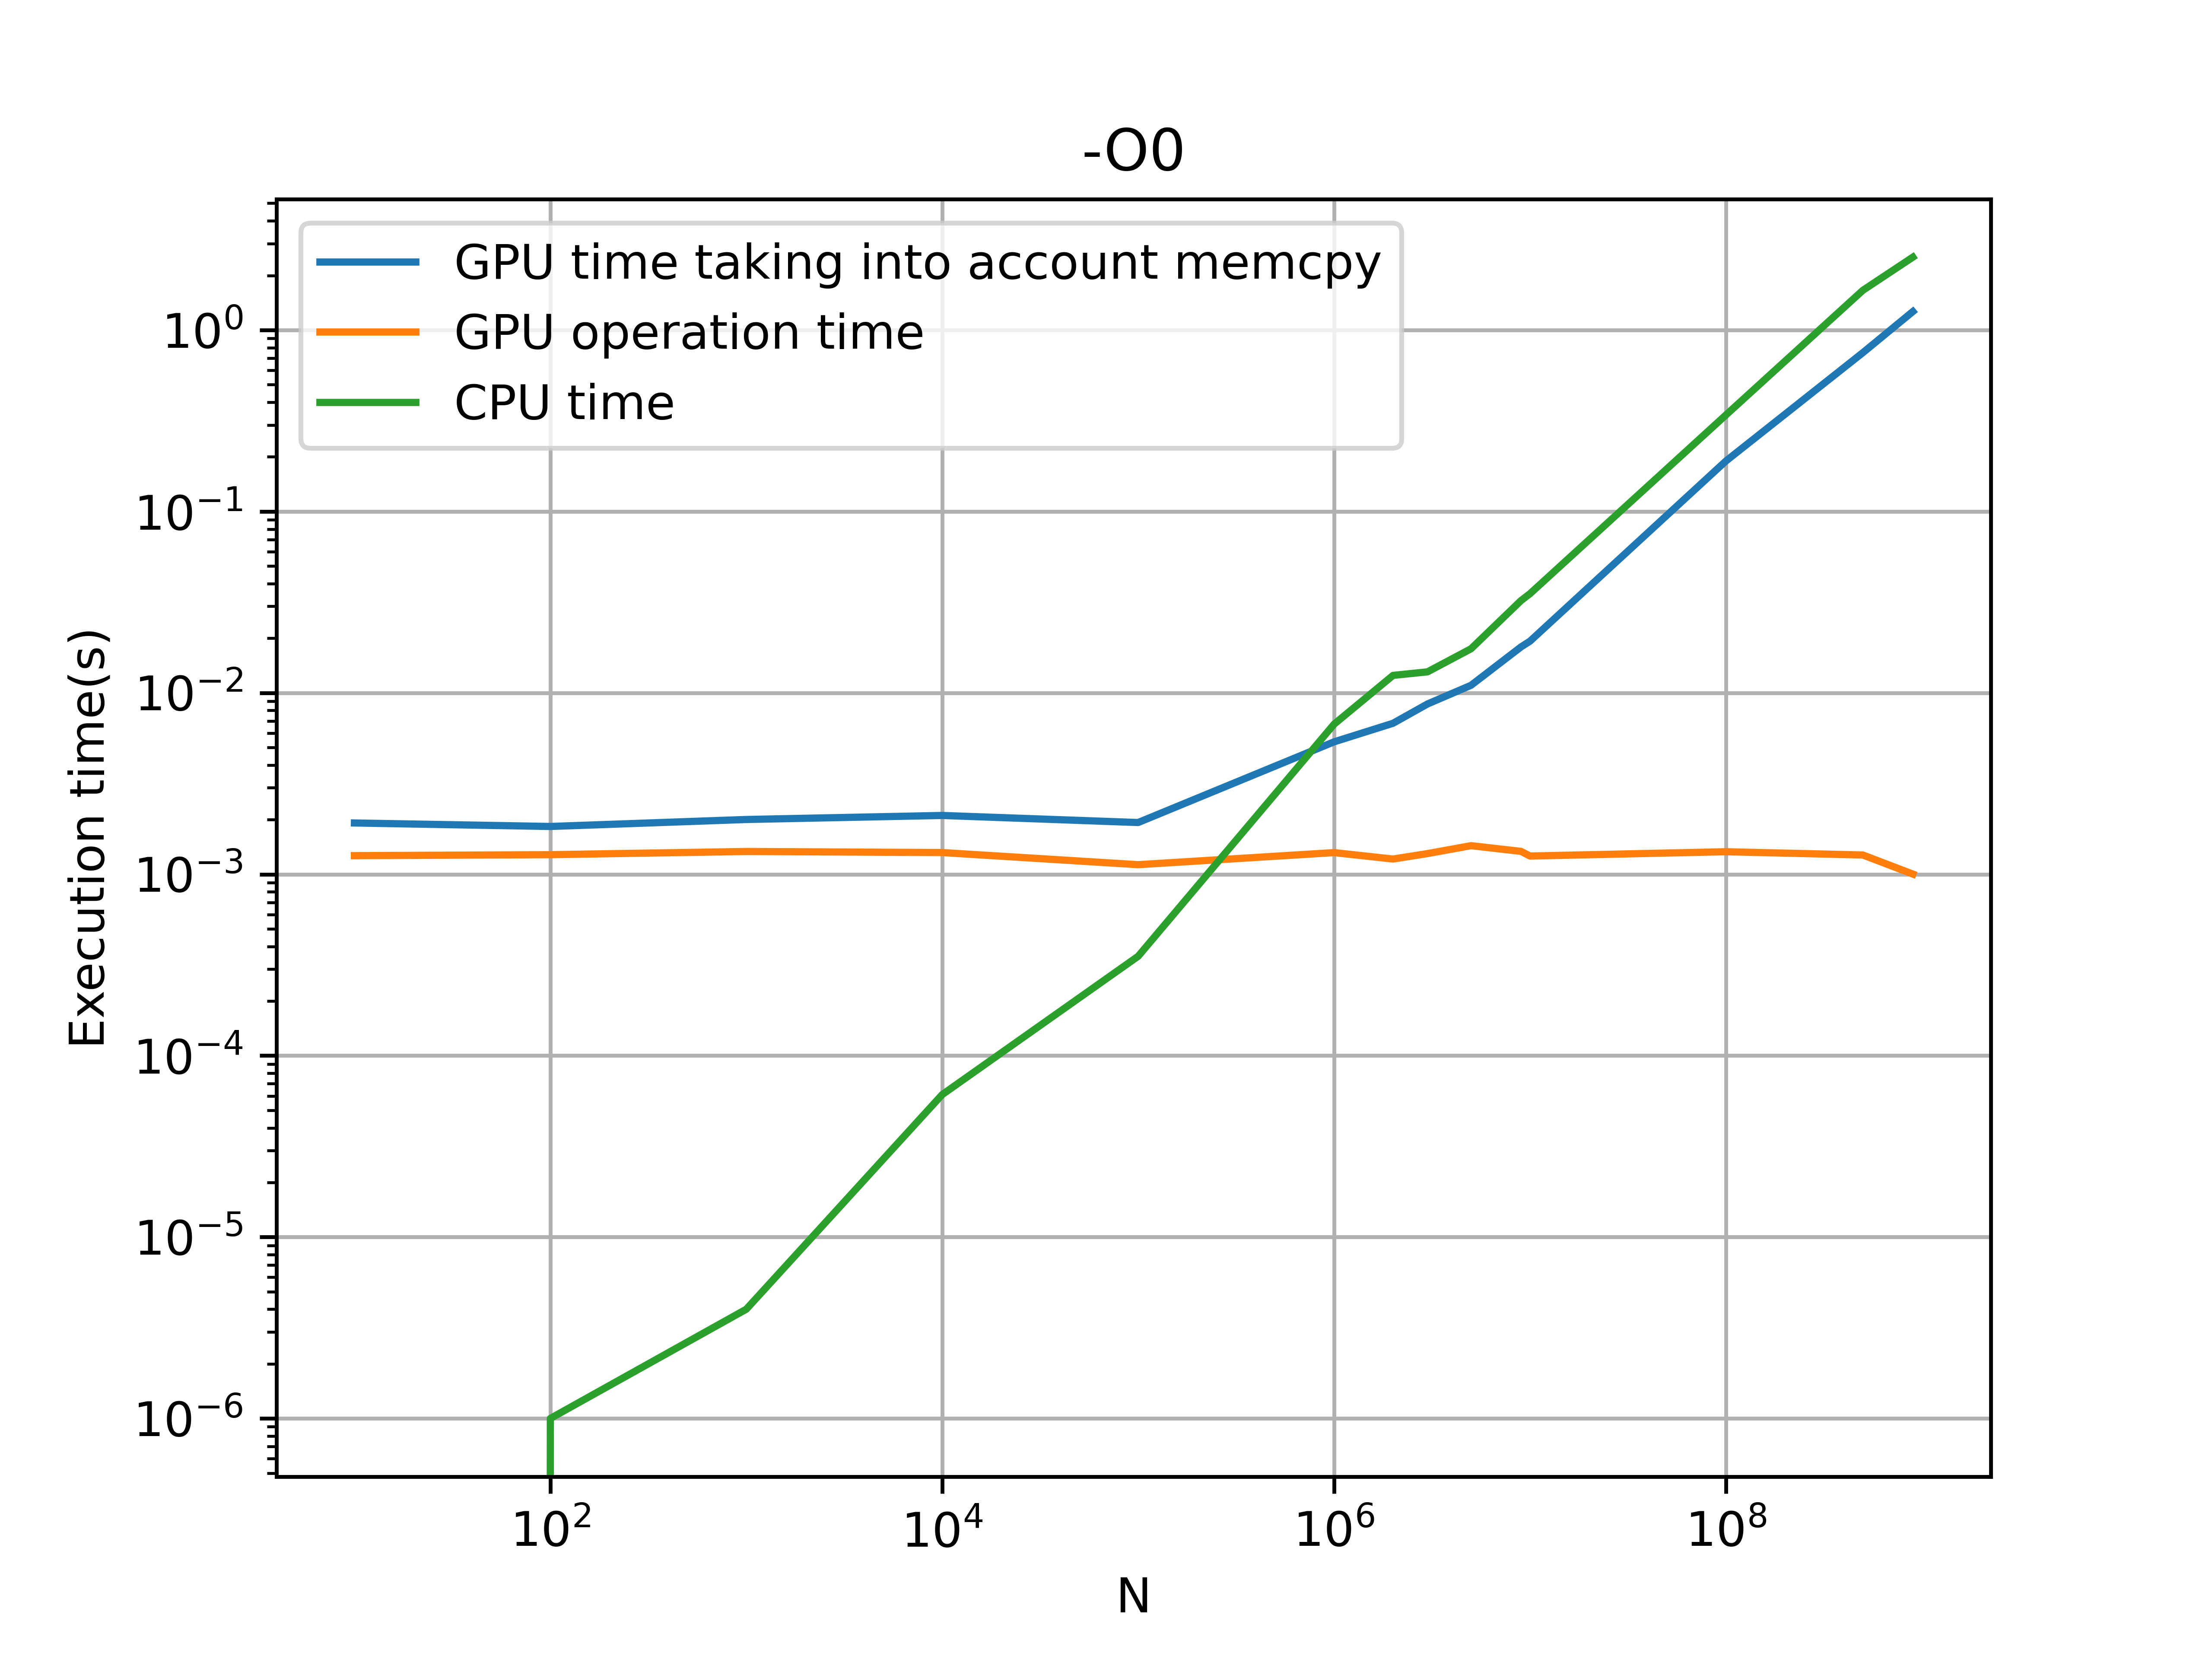
\includegraphics[width=0.8\textwidth]{O0.png}
\caption{K80:2 configuration}
\label{fig:bandwidthTest}
\end{figure}


\begin{figure}[H]
  \centering
  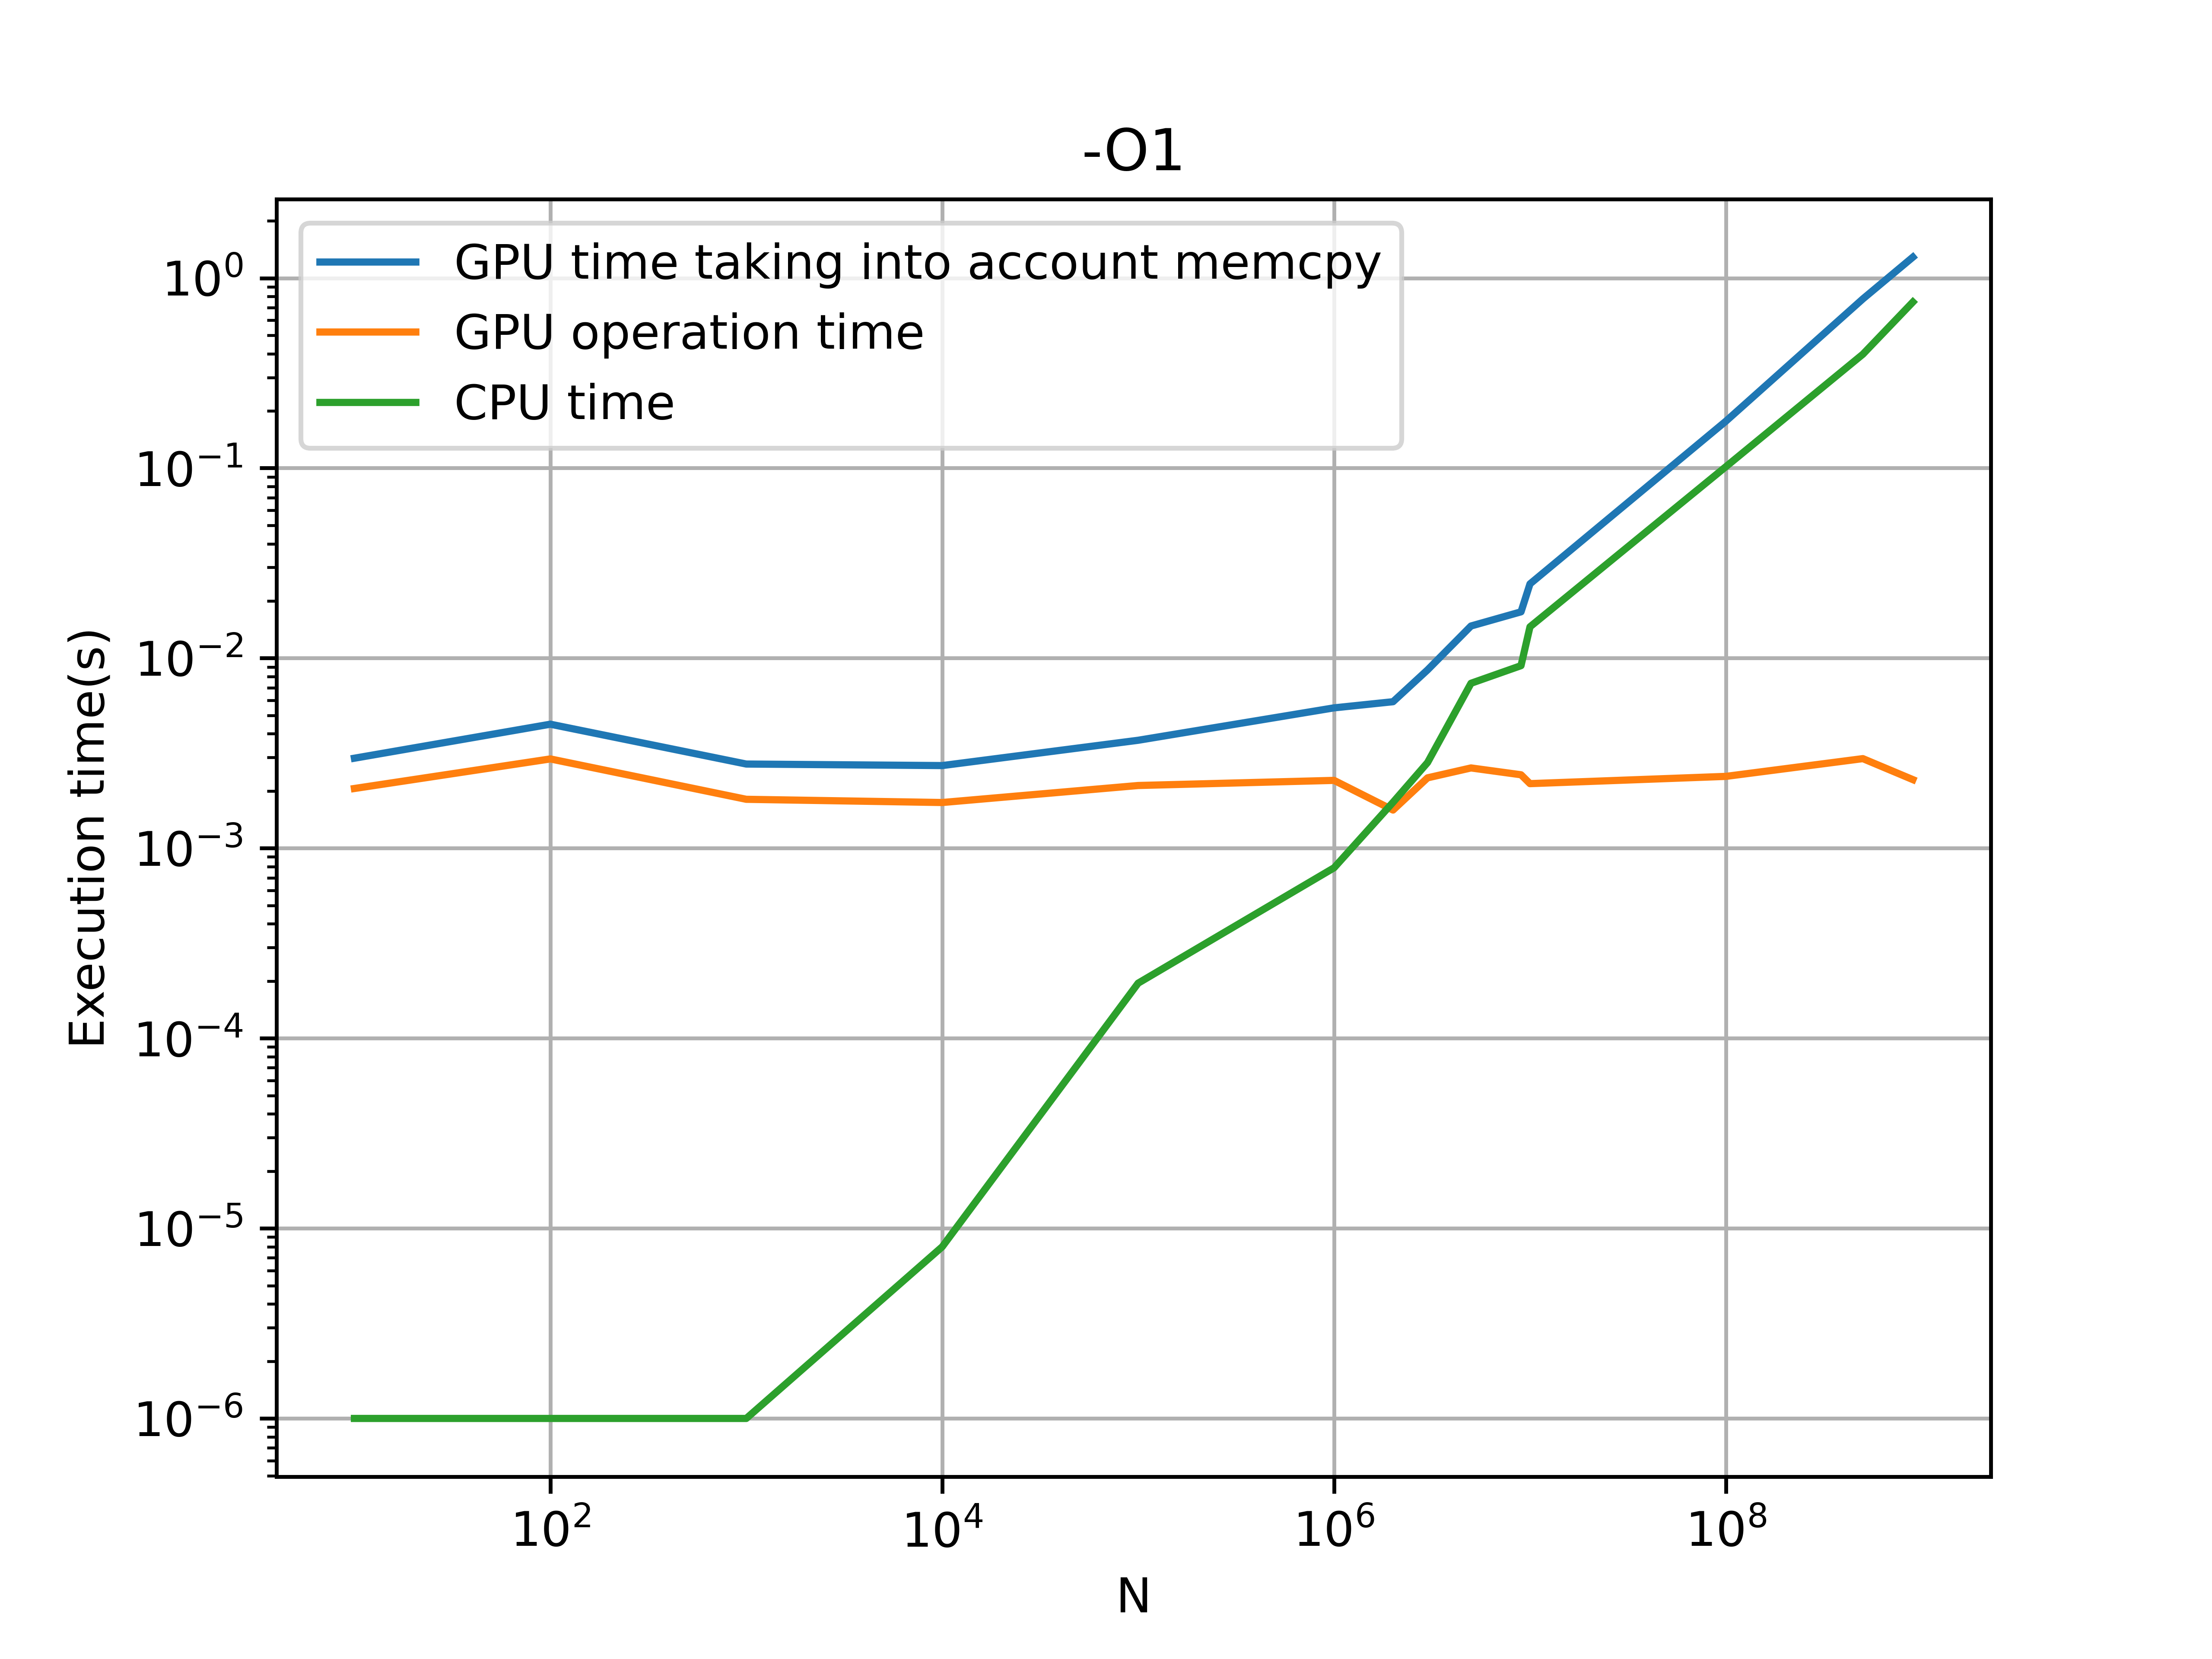
\includegraphics[width=0.8\textwidth]{O1.png}
  \caption{K80:2 configuration}
  \label{fig:bandwidthTest}
  \end{figure}
  

\end{document}

